\documentclass[10pt]{article}
\usepackage[utf8]{inputenc}
\usepackage[swedish]{babel}

\def\ordf{Edvard Carlsson}
\def\kon{Mattias Lundström}
\def\krog{Davida Åström}
\def\fvc{Henrik Ramström}
\def\enuordf{Jakob Pettersson}
\def\sreordf{Lina Samnegård}
\def\sexm{Theo Nyman}
\def\ent{Saga Åslund}
\def\cafem{Jonathan Benitez}
\def\oph{Stephanie Bol}

\def\doctype{Handlingar} %ex. Kallelse, Handlingar, Protkoll
\def\mname{Höstterminsmötet} %ex. styrelsemöte, vårterminsmöte
\def\mnum{HTM/19} %ex S02/16, E01/15, VT/13
\def\date{2019-11-XX} %YYYY-MM-DD
\def\docauthor{\ordf}

\def\mtime{17:15}
\def\place{E:X}

\usepackage{../../_sektion-handlingar/e-handlingar-sek}
\usepackage{../../e-mote}
\usepackage{../../../../e-sek}

\begin{document}

\firstpage{{\doctype} till {\mname} {\mnum}}{{\date} {\mtime} i {\place}}

\tableofcontents
\newpage

\subfile{../../_sektion-handlingar/_other/guide}
\newpage

\section{Dagordning}
\subsection{Tid och plats}
\tidplats

\subsection{Föredragningslista}
\begin{paralist}
    \pli{TaFMÖ}{}
    \pli{Val av mötesordförande}{}
    \pli{Val av mötessekreterare}{}
    \pli{Godkännande av tid och sätt}{}
    \pli{Val av två justeringspersoner}{}
    \pli{Adjungeringar}{}
    \pli{Godkännande av dagordningen}{}
    \pli{Föregående sektionsmötesprotokoll}{}
    \pli{Meddelanden}{}
    \pli{Beslutsuppföljning}{}
    \pli{Utskottsrapporter}{}
    \pli{Uppföljning av verksamhetsplan}{}
    \pli{Ekonomisk rapport}{}
    \pli{Uttag ur Sektionens fonder sedan förra terminsmötet}{}
    \pli{Resultatrapport från första halvan av verksamhetsåret}{}

    \pli{Behandling av motioner}{}
        \begin{paralist}
          \pli{Döp om Kontaktor till Kommunikator}{}
        
        \end{paralist}
    \pli{Behandling av propositioner}{}
        \begin{paralist}
            \pli{Budgetförslag för 2019}{}
            \pli{Verksamhetsplansförslag för 2019}{}
            \pli{XXX}{}
           
        \end{paralist}
    \pli{Övrigt}{}
    \pli{TaFMA}{}
\end{paralist}

\begin{signatures}{2}
    \emph{I Sektionens tjänst}
    \signature{\ordf}{Ordförande}
    \signature{\sekr}{Kontaktor}
\end{signatures}

\subfile{../_other/ekonomisk_rapport}
\newpage
\addcontentsline{toc}{subsection}{Balansrapport}
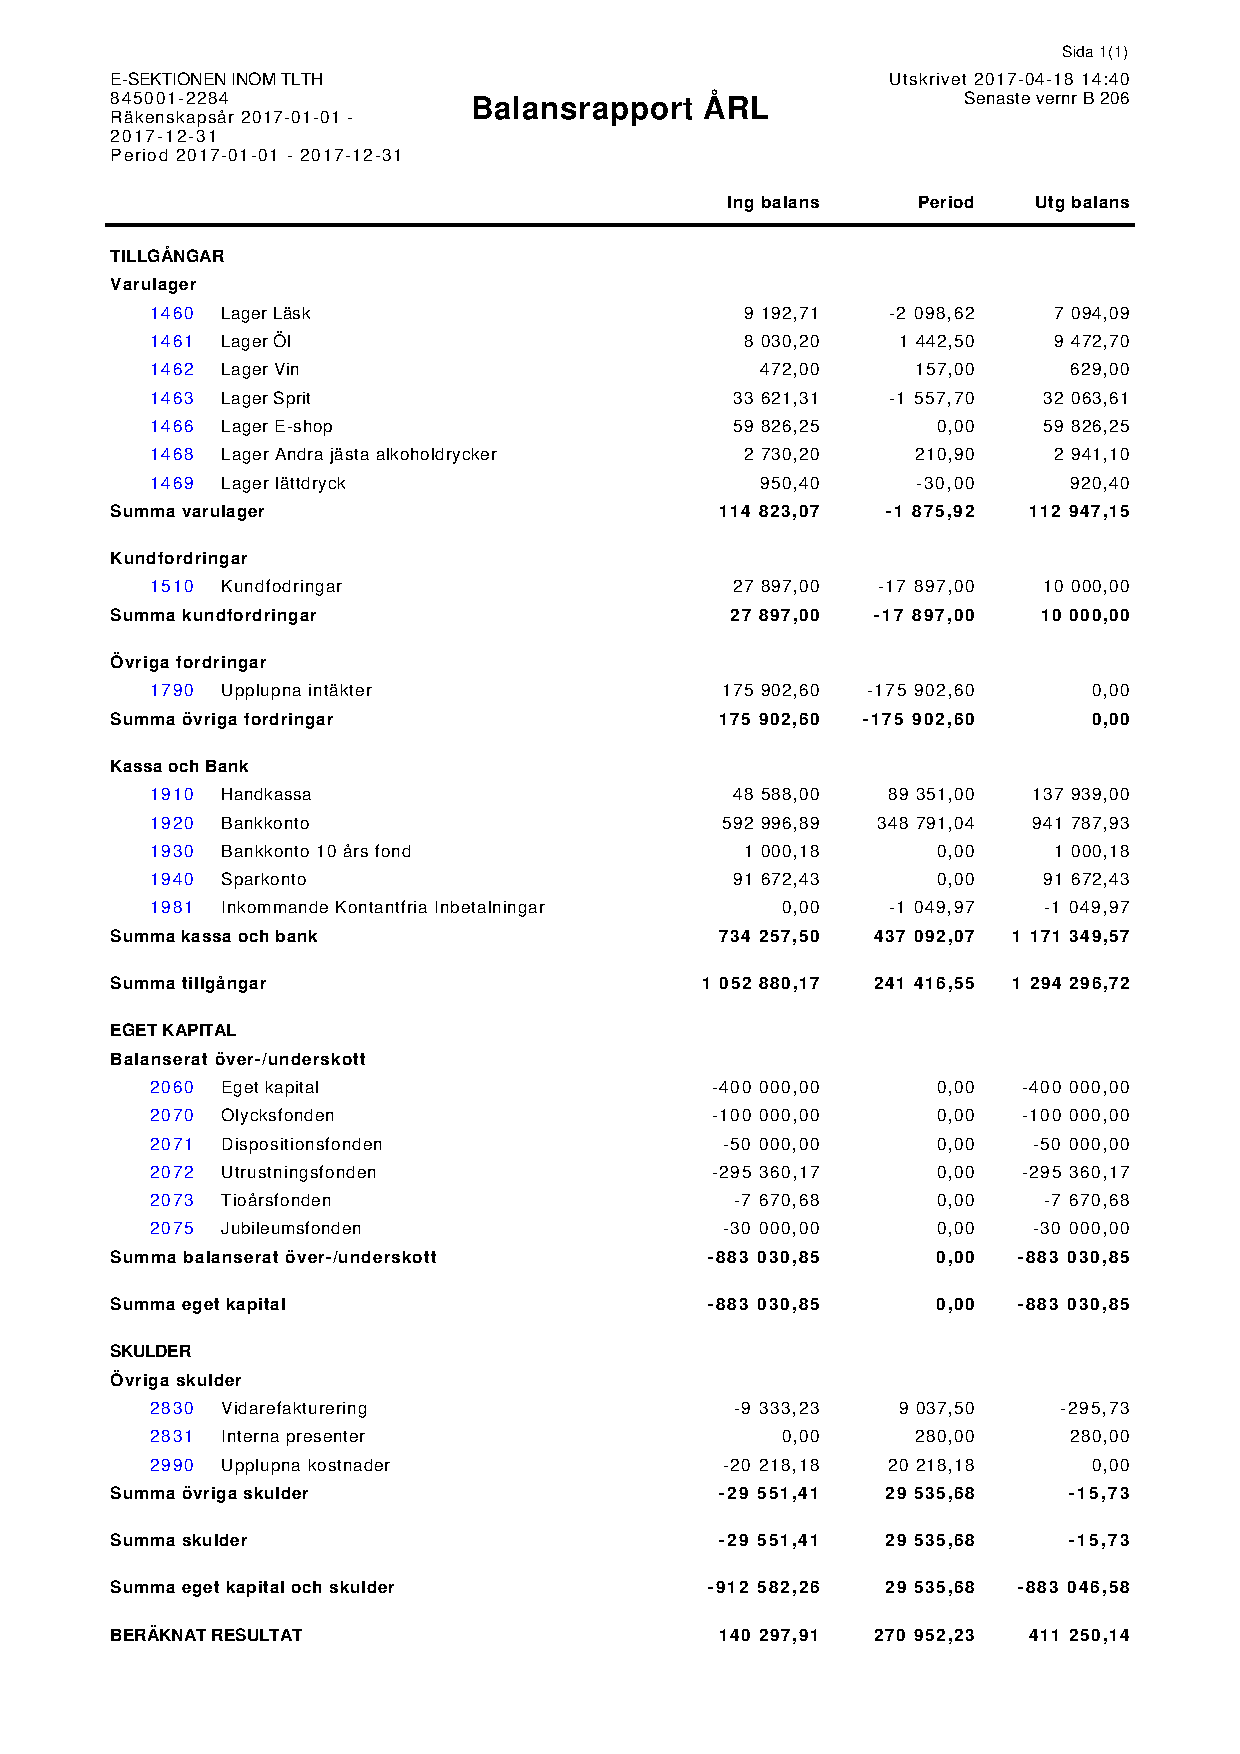
\includepdf[pages=1]{../_res/balansrapport.pdf}

\subfile{../_other/uttag}
\newpage

\begin{supersection}{Beslutsuppföljningar}{}
    \subsection{Överblick}
    \begin{busek}
    \beslutsek{HT/16}{Fanbärare behöver längre påle}{Emil Harvig}{\SI{500}{kr} till inköp av en rundstav, benämnd som påle i vissa sammanhang}{HTM/19}

    

    \end{busek}

    \newpage
    \subfile{../beslutsuppf/XXX}
   

\end{supersection}

\begin{utskottsrapporter}
    \subfile{../utskottsrapporter/cm}
    \subfile{../utskottsrapporter/e6}
    \subfile{../utskottsrapporter/enu}
    \subfile{../utskottsrapporter/fvu}
    \subfile{../utskottsrapporter/infu}
    \subfile{../utskottsrapporter/km}
    \subfile{../utskottsrapporter/noju}
    \subfile{../utskottsrapporter/nollu}
    \subfile{../utskottsrapporter/sre}
    \subfile{../utskottsrapporter/styrelsen}
    \subfile{../utskottsrapporter/vb}
\end{utskottsrapporter}

\begin{supersection}{Verksamhetsplaner}{}
   \subfile{../verksplan/2019}
\end{supersection}

\begin{supersection}{Uppföljningar av verksamhetsplaner}{}
    \subfile{../verksamhetsplanuppf/2019-vt}
    \subfile{../verksamhetsplanuppf/2019-ht}
\end{supersection}

\begin{motioner}
\subfile{../motion/}
\subfile{../motionssvar/XXX}

\end{motioner}

\begin{propositioner}
  \subfile{../prop/XXX}
 
\end{propositioner}

\begin{supersection}{Halvårsbokslut 2019}{}
    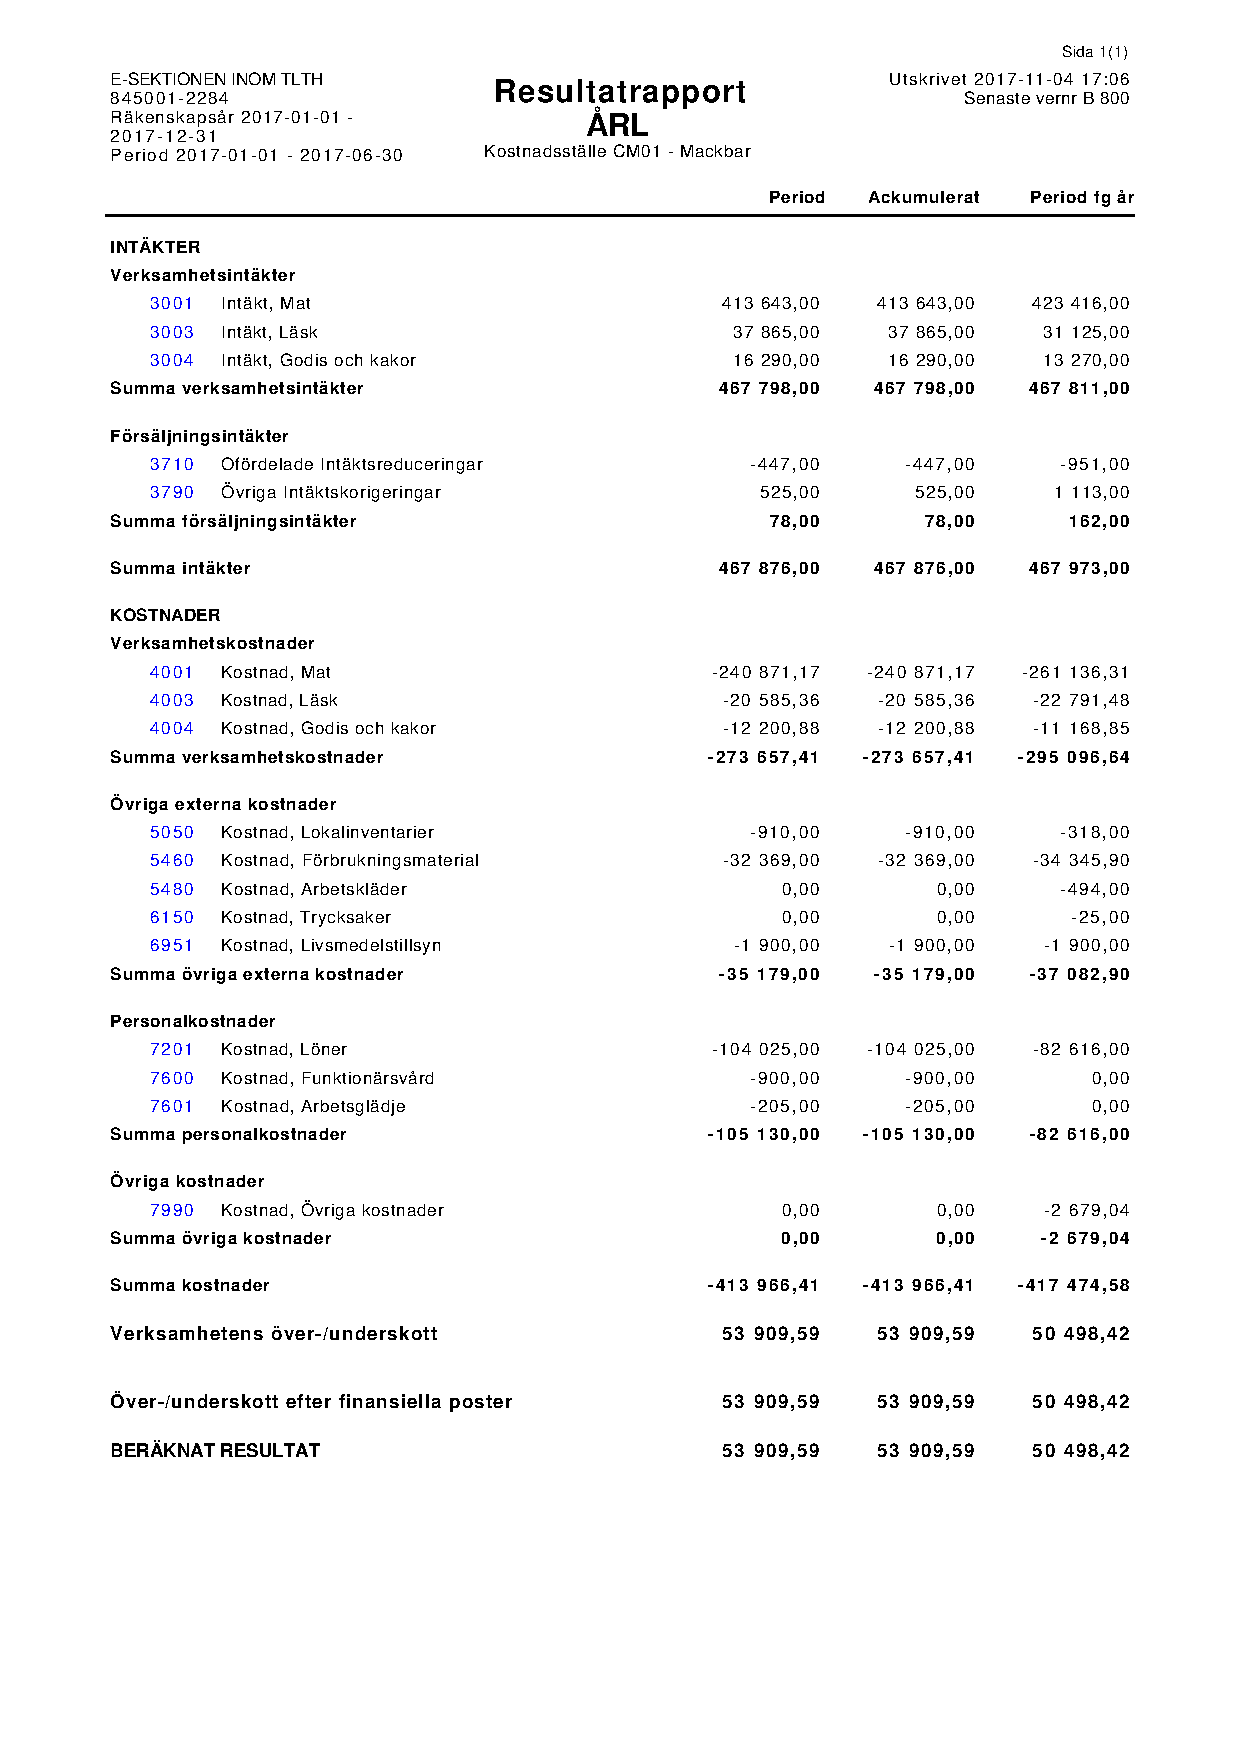
\includepdf[pages=-]{../_res/bokslut/halvarsbokslut.pdf}
\end{supersection}

\end{document}
